\section{Task 2}\label{sec:task2}

The goal of the second task is to implement a software to quantify global differences between ensembles and to identify variance along the sequence. The input of this task is a file containing the features of one or more PED ensemble.

\subsection{Ensembles features}
Relationships between different ensambles will be identified considering the structural features of single ensemble using the features file of the task 1.

At the begining, the software extracts the features for each ensamble (multiple conformations):
\begin{itemize}
\item Radius of gyration.
\item Secondary structure entropy for each position acrossensemble conformations
\item Median ASA for each position across ensemble conformations using the model ASA .
\item Median RMSD using rotate-translation matrices for each model.
\item Median distance of each pair of equivalent positions. It consider the matrix columns of conformation distance matrices.
\item Standard deviation of the distance of each pair of equivalent positions.
\end{itemize}


\subsection{Global metric}
%-spiegazione metriche locali e globali, descrizione immagine con significato e osservazioni biologiche

Distance between ensembles
\begin{figure}[H]
	\begin{minipage}[b]{0.9\textwidth}
		\centering
		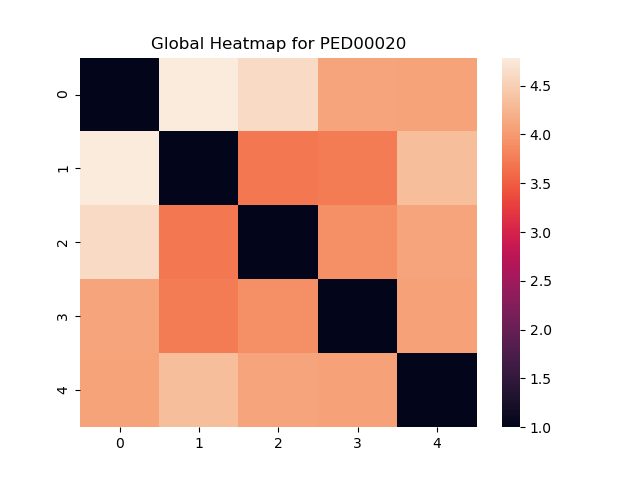
\includegraphics[width=\textwidth]{PED00020_heatmap.png}
		\caption{Heatmap of all the model.}
		\label{heatmap}
	\end{minipage}
	\hfill
	\begin{minipage}[b]{0.9\textwidth}
		\centering
		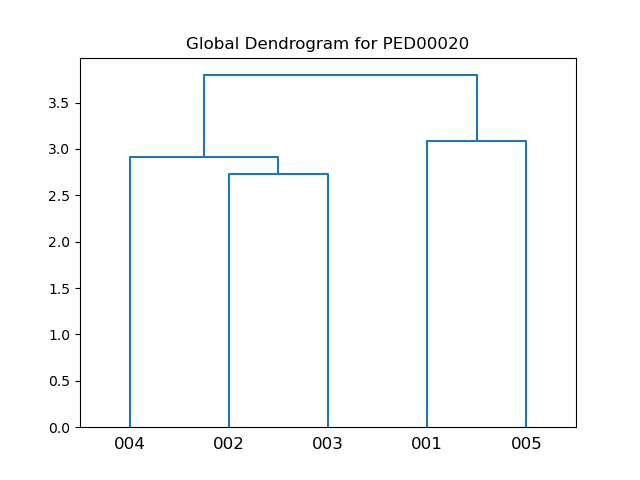
\includegraphics[width=\textwidth]{PED00020_dendrogram.png}
		\caption{Dendrogram of all the model.}
		\label{dendrogram}
	\end{minipage}
\end{figure}



\subsection{Local metric}
Plot of ensemble features
\begin{figure}[H]
	\begin{minipage}[b]{0.9\textwidth}
		\centering
		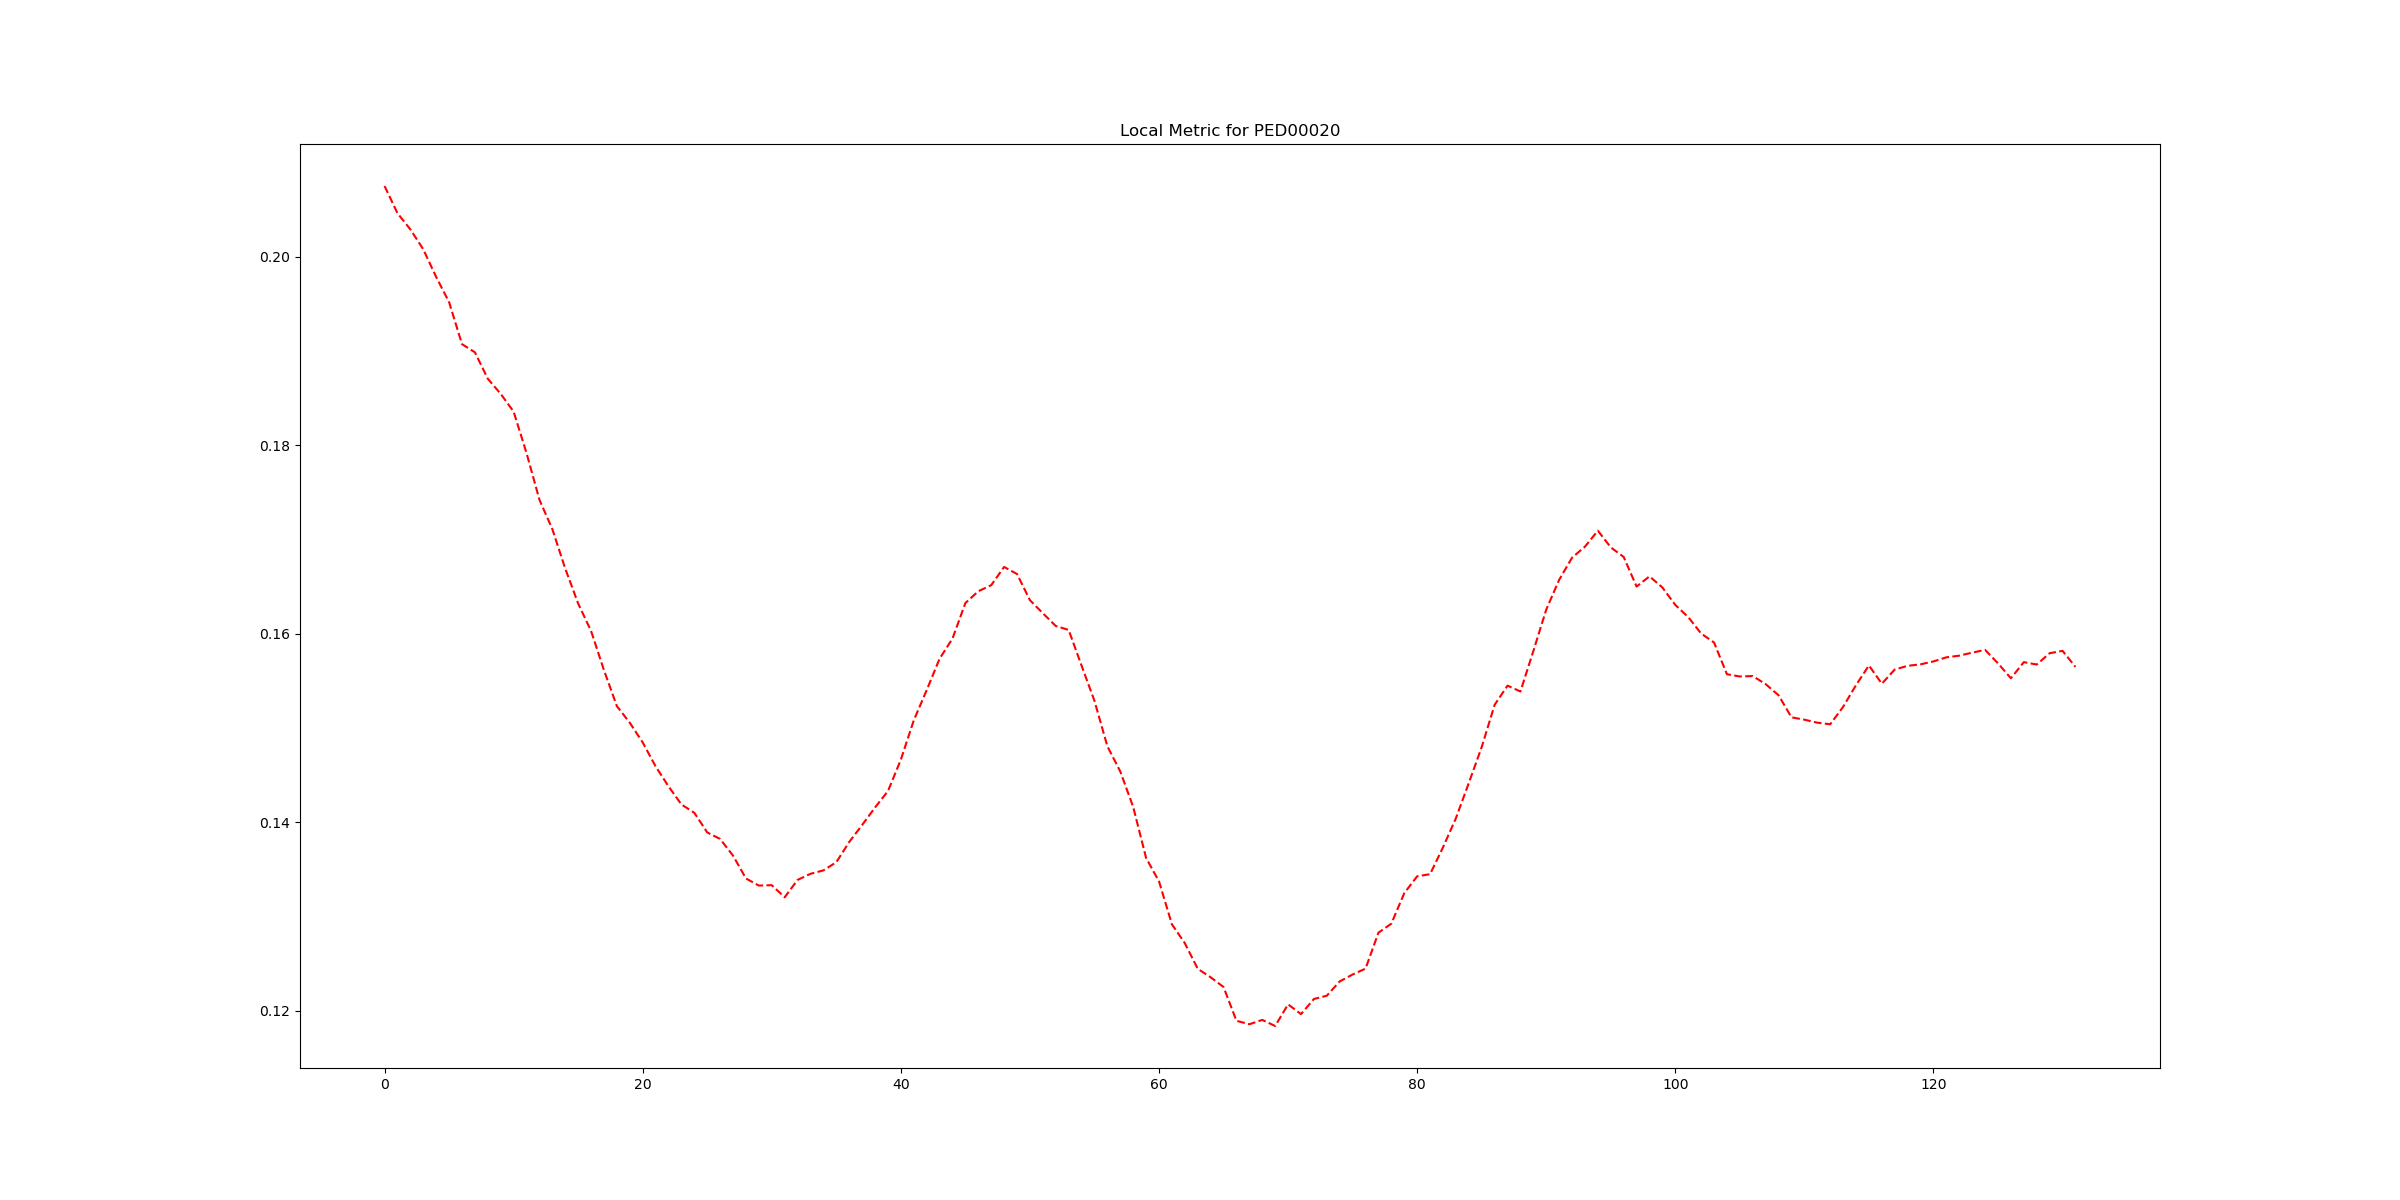
\includegraphics[width=\textwidth]{PED00020_local.png}
		\caption{Plot of local features.}
		\label{plot}
	\end{minipage}	
\end{figure}